\documentclass[10pt,conference]{IEEEtran}

\usepackage{cite}
\usepackage{amsmath,amssymb,amsfonts}
\usepackage{amsthm}
\usepackage{algorithm}
\usepackage{algpseudocode}
\usepackage{booktabs}
\usepackage{graphicx}
\usepackage{xcolor}
\usepackage{array}
\usepackage{tabularx}
\usepackage{multirow}
\usepackage{url}
\usepackage{tikz}
\usetikzlibrary{positioning,arrows.meta,calc,fit,shapes.geometric,patterns}
\usepackage{pgfplots}
\pgfplotsset{compat=1.18}

\newtheorem{definition}{Definition}
\newtheorem{theorem}{Theorem}
\newtheorem{lemma}{Lemma}
\newtheorem{proposition}{Proposition}
\newcommand{\Act}{\mathcal{A}}
\newcommand{\Rel}{\mathcal{R}}
\newcommand{\Obl}{\mathcal{O}}
\newcommand{\Suit}{\mathcal{S}}
\newcommand{\unknown}{\ensuremath{\mathsf{UNKNOWN}}}
\newcommand{\noaction}{\ensuremath{\mathsf{NO\_ACTION}}}
\newcommand{\upgrade}{\ensuremath{\mathsf{UPGRADE}}}
\newcommand{\alternative}{\ensuremath{\mathsf{ALTERNATIVE}}}
\newcommand{\notarget}{\ensuremath{\mathsf{REPAIR\_NO\_TARGET}}}
\newcolumntype{Y}{>{\raggedright\arraybackslash}X}
\newcolumntype{Z}{>{\centering\arraybackslash}X}
\newcommand{\tblfont}{\footnotesize}
\newcommand{\figbody}{\rmfamily\footnotesize}
\newcommand{\figsmall}{\rmfamily\footnotesize}
\newcommand{\figvalue}{\rmfamily\footnotesize}
\definecolor{cmbInk}{RGB}{27,31,36}
\definecolor{cmbBlue}{RGB}{43,82,125}
\definecolor{cmbTeal}{RGB}{43,125,116}
\definecolor{cmbGold}{RGB}{158,116,49}
\definecolor{cmbRose}{RGB}{151,75,82}
\definecolor{cmbMist}{RGB}{239,245,249}
\definecolor{cmbMint}{RGB}{237,247,244}
\definecolor{cmbWarm}{RGB}{248,244,235}
\definecolor{cmbRule}{RGB}{196,202,205}
\tikzset{
  rwPanel/.style={draw=cmbRule, rounded corners=2.2pt, line width=.55pt,
    align=center, fill=cmbMist, font=\figbody, text=cmbInk,
    inner xsep=1.8pt, inner ysep=1.0pt,
    text height=1.35ex, text depth=.28ex},
  rwPanelB/.style={rwPanel, fill=cmbMint},
  rwPanelC/.style={rwPanel, fill=cmbWarm},
  rwFlow/.style={-{Latex[length=1.7mm]}, line width=.72pt,
    draw=cmbBlue, line cap=round, line join=round},
  rwSoft/.style={line width=.45pt, draw=cmbGold, dashed,
    line cap=round, line join=round},
  rwLabel/.style={font=\figsmall, text=black!62, align=center,
    inner sep=.35pt, text height=1.2ex, text depth=.25ex}
}

\title{When Security Advisories Change Repair Decisions}
\author{\IEEEauthorblockN{Anonymous Author(s)}}

\begin{document}

\maketitle

\begin{abstract}
Security advisories that name the same vulnerability often disagree in affected ranges, repair targets, or remediation guidance. Existing comparisons largely stop at identifiers and version constraints, but a developer running release $v$ needs to know whether two claims prescribe the same repair action for that release. We present \emph{RepairWitness}, a conservative semantics and certificate system for this question. It maps each claim--release pair to a partial action trace, treats unresolved evidence as abstention, converts concrete action differences into release obligations, and synthesizes a small real-release suite that witnesses every divergence. The synthesis problem is weighted redundant multicover; we give exact, bounded, interval-structured, and approximation algorithms whose certificates are checked independently of the optimizer. On a frozen 2021 SafetyDB benchmark whose source bytes are digest-validated rather than redistributed, 570 of 602 claim-pair comparisons induce different actions, and the 97 divergent groups require a median of two witness releases rather than 23 when every witness is retained. A redistributable GHAD/PyPA overlap fixture separately gives source-level construct evidence: three advisory pairs have identical affected-release sets but different repair actions. Exact certificates agree with an independent HiGHS formulation on all groups. Across 544 controlled instances, three independent solving paths agree, every certificate replays, and deliberate certificate mutations are rejected. The interval algorithm handles 100,000 releases and obligations in 1.48 seconds, and a 50-instance OR-Library run reaches 49 known optima under a four-second per-instance budget. RepairWitness turns opaque advisory disagreement into compact, reproducible evidence about when public security guidance changes a repair decision.
\end{abstract}

\begin{IEEEkeywords}
security advisories, vulnerability remediation, software ecosystems, semantic equivalence, certified optimization, set multicover
\end{IEEEkeywords}

\section{Introduction}
Software supply-chain security increasingly depends on public vulnerability records. Package managers, software-composition-analysis tools, and repository hosting platforms translate these records into alerts and upgrade suggestions. Dependabot alerts surface vulnerable dependencies in hosted repositories~\cite{githubDependabotAlerts}; OSV-Scanner checks projects against OSV records~\cite{osvScannerDocs}; Grype scans container images and filesystems~\cite{grypeDocs}; Snyk CLI scans open-source dependencies~\cite{snykCliOpenSource}. Yet public curations do not merely duplicate one another: they may encode different affected ranges, identify different patched releases, preserve or omit alternative mitigations, or disagree about whether any public repair target exists. Prior work has documented inconsistent vulnerability reports and substantial variation among composition-analysis tools \cite{dong2019inconsistencies,imtiaz2021sca}; ecosystem studies further show that vulnerable dependencies propagate widely and that developers delay updates even after disclosure \cite{zimmermann2019npm,kula2018updates,zerouali2022impact,liu2022dvgraph}. What remains missing is an executable unit of comparison.

For a developer running release $v$, the operational question is not whether two JSON objects are equal. It is whether they imply the same action: keep $v$, upgrade to a source-supported release, apply a non-version mitigation, repair without an available public target, or abstain because the public evidence is incomplete. Range equality can be too coarse in both directions. Syntactically different ranges can select the same released versions, while identical affected sets can still name different repair targets. Conversely, a textual difference outside the package's actual release history need not change any developer decision. Version syntax is itself ecosystem-specific: Python and SemVer-derived ecosystems define different operators and compatibility conventions \cite{pep440,semver,cargoSemver}. Maven, Go modules, and NuGet add distinct ordering and range corner cases \cite{mavenVersions,goModules,nugetVersions}.

We introduce \emph{repair-action equivalence}: equality of partial action traces over a digest-bound public release universe. The semantics is conservative in two important ways. First, a curation's ``fixed'' or ``patched'' version is a source-supported \emph{repair anchor}, not a claim that the version is universally safe, compatible, or maintained. Second, uncertainty is an abstention rather than a sixth action: an unresolved cell cannot make two claims equivalent or divergent.

Action traces expose a second challenge. A group containing $k$ claims may induce $\binom{k}{2}$ divergent edges, and each edge may differ on many releases. Retaining every release--edge pair is redundant and difficult to audit. RepairWitness instead constructs an \emph{action-separating suite}: a small set of actual releases such that every concrete divergent edge has the requested number of selected witnesses. Execution costs permit expensive releases to be penalized; witness demands permit resilience to unavailable releases. The general problem is weighted set multicover. Security-advisory traces additionally exhibit ordered structure: many witness sets are intervals in release order. We exploit that structure with a polynomial right-endpoint algorithm for unit costs and an exact primal--dual certificate for the weighted consecutive-ones case.

The key design principle is \emph{producer/checker separation}. The optimizer may use reductions, dynamic programming, branch-and-bound, greedy approximation, or an external MILP backend. A much smaller checker re-normalizes the original obligations, recomputes their digest, verifies the selected witnesses, recomposes component bounds, and rejects unsupported proof kinds. Thus, a result remains auditable without trusting the search implementation.

Figure~\ref{fig:pipeline} summarizes the evidence chain. Claims and real releases produce partial action traces; concrete differences become obligations; synthesis chooses releases; and a checker replays the resulting certificate against the original obligations. The evidence is deliberately layered: SafetyDB is a digest-validated historical case study, while the public-overlap, synthetic, controlled, and OR-Library layers are redistributable replay surfaces that do not depend on those source bytes.

\begin{figure}[t]
\centering
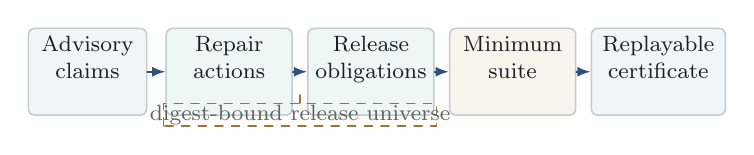
\begin{tikzpicture}[x=1mm,y=1mm]
\node[rwPanel,minimum width=15mm,minimum height=11mm] (claims) at (7.5,8.8) {Advisory\\claims};
\node[rwPanelB,minimum width=16mm,minimum height=11mm] (sem) at (25.5,8.8) {Repair\\actions};
\node[rwPanelB,minimum width=16mm,minimum height=11mm] (obl) at (43.5,8.8) {Release\\obligations};
\node[rwPanelC,minimum width=16mm,minimum height=11mm] (solve) at (61.5,8.8) {Minimum\\suite};
\node[rwPanel,minimum width=17mm,minimum height=11mm] (cert) at (80,8.8) {Replayable\\certificate};
\draw[rwFlow] (claims) -- (sem);
\draw[rwFlow] (sem) -- (obl);
\draw[rwFlow] (obl) -- (solve);
\draw[rwFlow] (solve) -- (cert);
\draw[rwSoft] (17.2,1.9) rectangle (51.8,4.8);
\node[rwLabel] at (34.5,3.35) {digest-bound release universe};
\draw[rwSoft] (34.5,4.8) -- (34.5,6.2);
\end{tikzpicture}
\caption{RepairWitness changes the comparison object from advisory syntax to developer actions, then compresses all concrete disagreements into a replayable release suite.}
\label{fig:pipeline}
\end{figure}

This paper makes four contributions:
\begin{enumerate}
  \item \textbf{Semantics.} A five-outcome partial repair-action model that distinguishes affectedness, repair anchors, non-version mitigations, and typed uncertainty.
  \item \textbf{Algorithms.} A weighted redundant action-separation formulation with sound kernelization, exact and bounded search, fixed-parameter dynamic programming, a logarithmic greedy bound, and polynomial algorithms for interval-structured obligations.
  \item \textbf{Certificates.} Digest-bound feasibility, lower-bound, component, interval, and primal--dual certificates checked independently of the optimizer.
  \item \textbf{Evidence.} A layered evaluation combining a digest-validated historical advisory benchmark, a redistributable public-overlap construct witness, differential and mutation testing, 100,000-release scalability, and all 50 standard OR-Library set-cover instances.
\end{enumerate}

\section{Background and Research Gap}
\subsection{Vulnerable dependencies and package ecosystems}
Research has established that package ecosystems are large, fast-moving dependency networks \cite{kikas2017structure,wittern2016dynamics,decan2017seven}. Freshness and technical-lag metrics quantify how far dependencies trail available releases \cite{cox2015freshness,decan2018lag}; semantic-versioning studies show that version numbers do not reliably prevent breaking changes \cite{raemaekers2014semver}. Security research has measured vulnerable dependency propagation \cite{zimmermann2019npm,zerouali2022impact,liu2022dvgraph,ruohonen2018python}, update behavior \cite{kula2018updates,derr2017updated,lauinger2017depend}, and the distinction between declared and actually reachable vulnerable code \cite{plate2015impact,ponta2018beyond,pashchenko2018counting}. Curated fix corpora and industrial tracking studies further show the importance of preserving exact source evidence \cite{ponta2019dataset,cadariu2015tracking}. These studies motivate release-aware reasoning but do not define when two vulnerability curations prescribe the same repair.

Public vulnerability infrastructures serve different purposes. CVE provides identifiers \cite{mell2002cve,cveprogram}; NVD enriches records and is itself a common empirical subject \cite{nvd,singla2023nvd}; CVSS summarizes severity \cite{cvss31}. GitHub Advisory Database \cite{ghad}, PyPA \cite{pypaadvisory}, Go \cite{govulndb}, RustSec \cite{rustsecdb}, and RubySec \cite{rubysecdb} preserve ecosystem-specific ranges and references. OSV provides a cross-ecosystem event schema \cite{osvschema}, while Package URL supplies package identities \cite{purlspec}. Report consistency, however, remains a known problem \cite{dong2019inconsistencies}; severity and exploit likelihood are separate constructs from remediation \cite{allodi2014severity,bozorgi2010beyond,sabottke2015social}.

Secure-update systems and in-toto show how signed metadata and supply-chain links can make update provenance auditable \cite{cappos2008mirror,torresarias2019intoto}. Package-manager attack studies and taxonomies show that dependency channels themselves are attack surfaces \cite{duan2021package,zahan2022weaklinks,ladisa2023taxonomy,ohm2020backstabber}. RepairWitness addresses a complementary failure mode: honest public curations can disagree about what a developer should do. Its output is not a replacement vulnerability database or a safety proof; it is compact evidence of the action differences already latent in public guidance.

\subsection{Why existing comparators are insufficient}
We distinguish four abstraction levels:
\begin{enumerate}
  \item \emph{raw equality}: serialized records are identical;
  \item \emph{structural equality}: normalized package, aliases, ranges, and targets match;
  \item \emph{affected-set equality}: the claims select the same members of a real release universe;
  \item \emph{action equivalence}: the claims induce the same concrete repair action at every release.
\end{enumerate}
Each level answers a useful but different question. Affected-set equality ignores target choice and alternative mitigations. Raw or normalized equality can over-report differences caused only by spelling, ordering, or equivalent interval encodings. The central empirical question is therefore whether moving to action semantics changes conclusions and, when it does, which releases expose the change.

\subsection{Relation to set cover}
Set cover and hitting set are classical NP-hard problems \cite{karp1972reducibility,garey1979computers}. Greedy algorithms achieve harmonic approximation guarantees \cite{johnson1974approximation,chvatal1979greedy,wolsey1982submodular,slavik1997tight}, and stronger exact or heuristic methods combine preprocessing, relaxation, and search \cite{balas1980setcover,caprara1999heuristic,rajagopalan1999primal}. Our novelty is not a better general worst-case ratio. It is (i) the software-engineering abstraction that turns action disagreements into release obligations, (ii) reductions and certificates that preserve the original evidence, and (iii) exploitation of consecutive-ones structure in ordered release traces. The relevant polyhedral fact is that consecutive-ones incidence matrices are totally unimodular \cite{fulkerson1965interval}; recognition of consecutive-ones matrices relates to PQ-trees \cite{booth1976pqtree}.

\section{Repair-Action Semantics}
\subsection{Claims, releases, and partial actions}
A normalized claim $c$ contains a package identity, an ecosystem-specific affectedness predicate $P_c$, zero or more source-supported target releases $T_c$, optional alternative guidance $M_c$, withdrawal state, and provenance. Let $U_p=\langle v_1,\ldots,v_n\rangle$ be the ordered public release universe for package $p$. The universe is part of the evidence: its response bytes, parser version, and canonical digest are recorded.

\begin{definition}[Repair action]
For claim $c$ and installed release $v\in U_p$, the partial action function is
\[
\begin{array}{rcl}
\Act(c,v,U_p) &\in& \mathcal{R},\\
\mathcal{R} &=&
\{\noaction,\ \upgrade(T),\\
&& \alternative(M),\\
&& \notarget,\\
&& \unknown(B)\}.
\end{array}
\]
If $v$ is not affected, the result is $\noaction$. If $v$ is affected and the claim names a valid public target, the result is $\upgrade(T)$. Explicit non-version guidance yields $\alternative(M)$; an acknowledged repair without a public target yields $\notarget$. Unsupported syntax, failed or empty universes, withdrawn ambiguity, invalid targets, and other unresolved evidence yield $\unknown(B)$ with a typed blocker $B$.
\end{definition}

The target set is deliberately source-relative. RepairWitness never rewrites $\upgrade(1.2)$ as ``1.2 is safe.'' The action means only that the claim supports 1.2 as its public repair anchor. This distinction prevents a curation comparison from silently making compatibility, support, or absence-of-vulnerability assertions.

\begin{definition}[Concrete divergence]
Claims $c_i$ and $c_j$ are concretely divergent at $v$ iff both actions are non-\unknown{} and $\Act(c_i,v,U_p)\neq\Act(c_j,v,U_p)$. Their witness set is
\[
\begin{aligned}
W_{ij}=\{v\in U_p\mid{}&\Act(c_i,v,U_p),\Act(c_j,v,U_p)\text{ concrete},\\
&\Act(c_i,v,U_p)\neq\Act(c_j,v,U_p)\}.
\end{aligned}
\]
They are action-equivalent iff every release with two concrete actions agrees and $W_{ij}=\varnothing$; comparisons with no jointly concrete cells are indeterminate rather than equivalent.
\end{definition}

This rule makes uncertainty monotone: adding unresolved cells cannot create evidence of agreement or disagreement. It also yields an auditable explanation for every edge: a release, two action traces, and their source fields.

\subsection{Version semantics and fail-closed evaluation}
RepairWitness dispatches version predicates to ecosystem-specific backends. Python uses PEP~440; npm, Cargo, Go, and related ecosystems use documented SemVer subsets; Maven and NuGet receive their own ordering and interval rules. Inputs outside the implemented contract fail closed rather than falling back to lexicographic ordering. The artifact includes conformance vectors and differential tests against independent libraries. This matters because strings such as prereleases, epochs, local versions, Maven qualifiers, and Go pseudo-versions can reverse naive comparisons.


\subsection{Worked action-trace example}
Table~\ref{tab:example} illustrates why affectedness, target choice, and uncertainty must remain separate. Claims $c_1$ and $c_2$ both mark releases before 1.10.0 affected and name 1.10.0 as the repair anchor; they are action-equivalent despite possible syntactic differences. Claim $c_3$ instead names 1.11.0. At 1.9.0, $c_1$ and $c_3$ are both affected but prescribe different upgrades. At 1.10.0, $c_1$ prescribes no action while $c_3$ still prescribes an upgrade. Either release witnesses their divergence; a minimum suite needs only one. If $c_3$ used unsupported version syntax, the corresponding cells would be \unknown{} and neither release could be selected as evidence.

\begin{table}[t]
\centering
\caption{Illustrative action traces over an actual release order. Claims $c_1$ and $c_2$ agree at every release, while $c_3$ changes the repair target and remains affected longer.}
\label{tab:example}
{\tblfont
\begin{tabularx}{\columnwidth}{@{}Yccc@{}}
\toprule
Claim & 1.9.0 & 1.10.0 & 1.11.0 \\
\midrule
$c_1$: affected $<1.10$, target 1.10 & $\upgrade(1.10)$ & $\noaction$ & $\noaction$ \\
$c_2$: equivalent encoding & $\upgrade(1.10)$ & $\noaction$ & $\noaction$ \\
$c_3$: affected $<1.11$, target 1.11 & $\upgrade(1.11)$ & $\upgrade(1.11)$ & $\noaction$ \\
\bottomrule
\end{tabularx}}
\end{table}

A real equivalence instance appears in the pinned PyPA and GitHub records for CVE-2020-29651 \cite{pypaadvisory,ghad}: both identify the Python package \emph{py}, list affected releases through 1.9.0, and anchor repair at 1.10.0. Their serialized records contain different links and database-specific fields, but their release-level repair actions coincide. This is precisely the type of false divergence removed by semantic projection.

\subsection{From traces to obligations}
For every divergent claim edge $e=(c_i,c_j)$, $W_e$ is a release obligation. Primary analysis uses unit cost $w(v)=1$ and unit demand $d(e)=1$. The general form permits positive integer execution cost $w(v)$ and redundancy $d(e)\geq 1$, e.g., requiring two witnesses so the explanation survives loss of one registry artifact.

\begin{definition}[Action-separating multicover]
Given obligations $\Obl=\{W_e\}_{e\in E}$, demands $d:E\rightarrow\mathbb{Z}_{>0}$, and costs $w:U_p\rightarrow\mathbb{Z}_{>0}$, find
\[
\min_{\Suit\subseteq U_p}\sum_{v\in\Suit}w(v)
\quad\text{s.t.}\quad
|\Suit\cap W_e|\geq d(e)\quad\forall e\in E.
\]
\end{definition}

The output suite is explanatory: each selected release may witness several edges, and each edge records the selected releases that discharge its demand.

\section{Certified Suite Synthesis}
\subsection{General solver}
The general problem is NP-complete by the unit-cost, unit-demand hitting-set special case. RepairWitness nevertheless solves the small, structured groups arising in advisory comparison exactly in practice. Its normalization sorts release and edge identifiers, validates costs and demands, removes duplicate witnesses, and binds the resulting object with canonical JSON and SHA-256 \cite{rfc8785}.

The kernel applies four sound transformations. \emph{Signature quotienting} groups releases covering the same residual obligations and keeps the cheapest deterministic representative. \emph{Forced propagation} selects a release when an edge's remaining witnesses equal its remaining demand. \emph{Obligation dominance} removes a row whose demand is implied by a stronger row with no larger residual support. Finally, the bipartite release--edge graph is split into independent connected components. Each transformation is recorded in kernel statistics so replay checks the original, not merely reduced, obligations.

For a component, the exact engine chooses between demand-state dynamic programming and deterministic best-first branch-and-bound. The DP state is the capped residual-demand vector, yielding $\prod_e(d(e)+1)$ states. Branch-and-bound starts from a greedy incumbent, branches on the tightest uncovered edge, and combines a packing bound with cost-per-uncovered-demand bounds. If a node budget expires, the smallest frontier lower bound and incumbent upper bound form a certified interval; completed components expose equality of bounds.

\begin{theorem}[General certificate soundness]
If the checker accepts a suite certificate, then (i) its selected releases satisfy every original obligation and demand, (ii) its objective equals the selected release cost, and (iii) the reported lower bound does not exceed the optimum while the reported upper bound does not fall below it. Equality certifies optimality.
\end{theorem}
\begin{proof}[Proof sketch]
The checker independently normalizes and hashes the problem; recomputes every selected-edge intersection; verifies forced selections and component partitioning; and checks each component's proof kind. DP completion enumerates all reachable capped-demand states. Branch-and-bound completion proves every pruned node is dominated by its admissible lower bound; bounded runs use the minimum live frontier bound. Additivity follows from disjoint component release and edge sets. Full arguments are in the supplement.
\end{proof}

The deterministic greedy baseline selects the release minimizing cost divided by newly satisfied demand, then reverse-deletes redundant choices. Standard charging gives an $H_Q$ approximation factor where $Q=\sum_e d(e)$ \cite{chvatal1979greedy,wolsey1982submodular}; no polynomial algorithm can improve the logarithmic worst-case threshold in general unless standard complexity assumptions fail \cite{feige1998threshold}. An independent exhaustive oracle handles small instances; a separate HiGHS MILP formulation checks larger ones.

\subsection{Ordered interval structure}
Release histories impose a total order. Many action divergences begin or end at a boundary, making $W_e$ a contiguous interval. For unit costs, the minimum redundant interval stabbing problem admits a direct algorithm: sort obligations by right endpoint and, whenever an interval lacks its demanded selected points, add the rightmost still-unselected releases inside it.

\begin{theorem}[Right-endpoint optimality]
For unit-cost interval obligations on a fixed release order, right-endpoint insertion returns a minimum-cardinality redundant action-separating suite.
\end{theorem}
\begin{proof}[Proof sketch]
Process intervals by nondecreasing right endpoint. When interval $I$ has deficit $q$, any feasible extension must add at least $q$ points in $I$. Replacing those points by the $q$ rightmost available points in $I$ cannot reduce coverage of any unprocessed interval, whose right endpoint is no earlier. Induction preserves an optimal extension after every step. A Fenwick tree counts selected points and a predecessor disjoint-set locates rightmost unselected points, giving $O((m+n+|\Suit|)\log n)$ time.
\end{proof}

For positive costs, the interval incidence matrix has the consecutive-ones property and is totally unimodular. We solve the bounded covering LP with $0\leq x_v\leq1$; integrality yields an optimal suite. A separate dual solve produces exact rational edge and cap weights. The checker verifies primal feasibility, dual feasibility, and equality between integer primal cost and the ceiling of the dual objective.

\begin{theorem}[Weighted interval certificate]
For interval obligations with integral costs and demands, an accepted RepairWitness primal--dual certificate proves global optimality.
\end{theorem}
\begin{proof}[Proof sketch]
Consecutive-ones matrices are totally unimodular \cite{fulkerson1965interval}; adding identity rows for upper bounds preserves total unimodularity. Integral right-hand sides therefore admit an integral optimal extreme point. Exact rational replay establishes weak duality and matching integer objectives, hence optimality.
\end{proof}


\subsection{Resilience and incremental maintenance}
A static minimum suite may be fragile if a selected release later disappears from a mirror or becomes expensive to execute. The demand function provides a direct robustness control: setting $d(e)=f+1$ guarantees that every obligation retains at least one selected witness after any $f$ selected releases fail, provided each obligation originally contains enough distinct witnesses. RepairWitness first checks this feasibility condition; it never duplicates one release to satisfy redundancy.

When claims or releases evolve, recomputing from scratch can cause unnecessary churn. The incremental mode takes a previously verified suite $\Suit_0$ and new obligations $\Obl'$. It preserves every still-valid release in $\Suit_0$, computes residual demands, and minimizes only the additional cost. A subsequent reverse-delete pass removes preserved releases that have become redundant. The result is optimal for the registered \emph{minimum-augmentation} objective, which lexicographically minimizes added cost and then final cost. This distinction is important: a globally smallest new suite could discard every old witness, defeating stable regression testing.

The certificate records the base-suite digest, surviving releases, residual obligations, and augmentation proof. Its checker first replays the old certificate, then confirms that every residual demand was computed against the surviving selection. Thus a stale or tampered base suite cannot silently authorize an incremental result. In the SafetyDB run, one-failure resilience is feasible for 67 of 97 divergent groups and stable augmentation applies to 72 groups.

\subsection{Independent checking algorithm}
Algorithm~\ref{alg:check} gives the checker core. It is intentionally simpler than the producer: it performs no search and trusts no cached reduction. Every acceptance decision is derived from the original normalized problem, the certificate payload, and exact arithmetic where available.

\begin{algorithm}[t]
\caption{Independent certificate replay}
\label{alg:check}
\begin{algorithmic}[1]
\Require original problem $P$, certificate $C$
\State $P'\gets\textsc{Normalize}(P)$; reject if $H(P')\neq C.\mathit{digest}$
\State reject unknown solver versions, algorithms, or proof kinds
\State recompute cost of $C.\mathit{selected}$ and compare with $C.\mathit{upper}$
\ForAll{obligations $e$ in $P'$}
  \State $X_e\gets C.\mathit{selected}\cap W_e$
  \State reject if $|X_e|<d(e)$ or recorded witnesses are outside $X_e$
\EndFor
\State recompute forced choices and connected components
\State reject unless component edge sets form a disjoint partition
\State verify each exact, bounded, DP, interval, or dual proof independently
\State reject unless component bounds and selections recompose globally
\State \Return accept
\end{algorithmic}
\end{algorithm}

Two details prevent common certificate bugs. First, the checker validates the \emph{original} obligation map; a sound reduction may justify search pruning, but it cannot redefine what counts as covered. Second, a proof-kind string is not decorative metadata. Each kind selects a distinct verification predicate, and the global kind must recompose from component kinds. The mutation campaign therefore includes an unbound-label case: accepting the label without the predicate would let a valid feasible selection masquerade as an optimality certificate.

\subsection{Certificate attack surface}
Certificates bind the solver version, normalized problem digest, selected releases, per-edge witnesses, costs, demands, kernel statistics, component bounds, and proof kind. Mutation tests alter each of these fields. The checker rejects digest substitution, unsupported versions, invalid selections, inconsistent bounds, and proof-kind recomposition. This separation is essential: testing only that the producer accepts its own output would leave shared-bug and stale-input failure modes undetected.

\section{Implementation and Evaluation Design}
The implementation keeps repair semantics, release acquisition, optimization, and replay checking as separate trust boundaries. Network acquisition enforces HTTPS, host allowlists, response-size and media-type limits, redirect revalidation, and atomic writes. Canonical payloads use sorted JSON; deterministic archives use sorted paths, fixed timestamps, fixed modes, and verified SHA-256 manifests. These choices follow reproducible-computing guidance on traceable analysis and executable claims \cite{peng2011reproducible,sandve2013ten,wilson2014best}. They also reflect artifact-review work that treats packaging, repeatability, and archival evidence as part of the scientific claim \cite{collberg2016repeatability,krishnamurthi2015artifact,ferro2018badging}.

We evaluate four questions:
\begin{description}
\item[RQ1:] Do public claims that share a package and CVE induce different concrete actions, and which comparators preserve that relation?
\item[RQ2:] How compact are exact action-separating suites, and do independent solvers agree?
\item[RQ3:] Are the algorithms and certificates correct under differential, metamorphic, and adversarial mutation tests?
\item[RQ4:] How do the specialized and general methods scale, including on an external standard set-cover benchmark?
\end{description}


\subsection{Engineering architecture}
The implementation separates evidence acquisition, repair-action semantics, optimization, and independent replay. Source adapters project upstream records into immutable normalized claims; registry adapters preserve successful, empty, and failed release-universe outcomes instead of deleting inconvenient packages. The semantic layer consumes only normalized claims and terminal release rows. The optimizer consumes only concrete witness obligations, so no \unknown{} cell can become a certificate witness.

This architecture is not required to solve set cover; it is required to make empirical security evidence auditable. Qualification checks bind source manifests, release ledgers, parser identities, validation samples, and replay evidence before observational results can be produced. A verifier recomputes the same digests without importing producer state. Changes to a source frame, validation sample, semantic implementation, baseline lock, or proof payload therefore invalidate the corresponding result. The same digest discipline binds paper tables to machine-readable receipts.

\subsection{Datasets and baselines}
\textbf{SafetyDB.} We use the frozen 2021.7.17 SafetyDB snapshot as a historical external advisory benchmark~\cite{safetydb}. Claims are grouped by normalized package and valid CVE; only groups with multiple records form edges. A digest-bound PyPI release-universe ledger preserves successful, empty, and failed package rows. The result manifest records exact input digests and all denominators. The original source bytes are not redistributed, so this layer supports digest-validated replay of the historical case study rather than source-level reconstruction by every reviewer.

\textbf{Public advisory overlap.} To avoid making one historical corpus carry the whole construct-validity burden, we include a redistributable GHAD/PyPA overlap fixture. It contains six public records, three paired edges, and frozen PyPI release universes for two packages. In all three pairs, affected-set equality says equivalent while the action relation finds a public-target or target-availability difference. The fixture is small by design: one source-level counterexample is enough to falsify affected-set sufficiency, but not to estimate how often the pattern occurs.

\textbf{Controlled validation.} Random but deterministic weighted multicover instances vary releases, edge density, costs, and demands. Separate interval instances vary order length, overlap, and redundancy. Each instance is solved by at least two independent formulations. Permuting input order tests determinism. Six certificate mutations test checker rejection.

\textbf{OR-Library.} We execute all 50 weighted set-cover instances in sets 4--6 and A--E from OR-Library \cite{beasley1990orlib}. Known optima are used only for evaluation. Baselines are cost-effectiveness greedy with reverse deletion, LP-guided rounding, and an independent HiGHS MILP limited to four seconds per instance. The evaluation fixes all 50 input files, their digests, selected solutions, and the result manifest.

\begin{table}[t]
\centering
\caption{Evaluation layers and independent checks.}
\label{tab:design}
{\tblfont
\begin{tabularx}{\columnwidth}{@{}p{1.35cm}p{2.2cm}Y@{}}
\toprule
Layer & Scale & Independent evidence \\
\midrule
SafetyDB & 1,246 CVE-tagged claims; 602 edges & affected-set and structural comparators; HiGHS; SetCoverPy; certificate replay \\
Public overlap & 6 public records; 3 edges & GHAD/PyPA source records; affected-set-equal but action-divergent replay \\
General & 192 weighted instances & exhaustive oracle; 32 HiGHS runs; permutation tests \\
Intervals & 160 unit-cost + 96 weighted & generic exact solver; rational primal--dual replay \\
Cross-cert. & 64 instances & separate proof bundles and strict checker \\
OR-Library & 50 public instances & known optima; three algorithms; frozen inputs \\
Scale & up to $10^5$ releases and obligations & separate solve and verification timing \\
\bottomrule
\end{tabularx}}
\end{table}

\subsection{Metrics and analysis discipline}
For RQ1 we report resolved divergence/equivalence and comparator agreement or mismatch relative to the action relation. For RQ2 we report exact objective, all-witness objective, compression $1-|\Suit|/|\cup_eW_e|$, solver agreement, and certificate validity. RQ3 reports objective agreement, replay counts, permutation invariance, and mutation detection. RQ4 reports approximation ratio to known optimum, runtime, node count, and memory. All denominators include failed or empty release-universe outcomes where applicable; unresolved cells are not silently discarded into equivalence.

\section{Results}
\subsection{RQ1: advisory differences are usually actionable}
The SafetyDB frame contains 1,246 CVE-tagged claims. After package--CVE grouping, 398 claims participate in 117 multi-record groups and form 602 pairwise edges. Of these, 570 (94.7\%) are resolved divergent and 32 (5.3\%) resolved equivalent. This high rate is a property of the historical duplicate-claim frame: it compares only package--CVE groups with multiple records, not random advisories or current ecosystem prevalence. It should be read as a stress case for historical curation consistency, while the public-overlap and synthetic layers test the construct without relying on that rate. The result is not merely textual churn: every divergent edge has at least one real release on which two concrete actions differ.

Raw and normalized structural equality each agree with the action relation on 583/602 SafetyDB edges (96.84\%) but report 19 false divergences. These cases have different encodings yet identical realized action traces. Affected-set equality reaches 602/602 on this historical dataset because the records predominantly encode one-sided upgrade boundaries; this is a corpus-specific fact, not a semantic theorem. The public-overlap fixture supplies the complementary source-level construct witness: all three included GHAD/PyPA pairs have equal affected-release sets but divergent repair actions, with 29--145 concrete witness releases per edge. We therefore treat SafetyDB and public overlap as two different evidence surfaces: the former estimates behavior in one historical corpus, while the latter falsifies affected-set sufficiency without estimating prevalence. Figure~\ref{fig:safety} visualizes the SafetyDB distributions.

\begin{figure}[t]
\centering
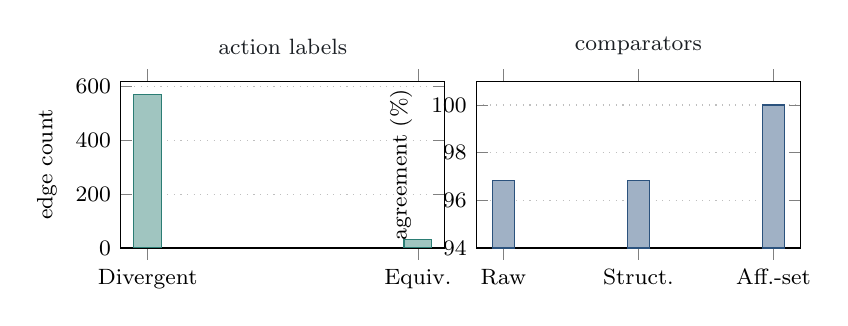
\begin{tikzpicture}
\begin{axis}[
  name=leftpanel,
  width=.47\columnwidth,height=3.7cm,
  ybar,bar width=10pt,
  symbolic x coords={Divergent,Equiv.},
  xtick=data,
  ylabel={edge count},
  ymin=0,ymax=620,
  ymajorgrids=true,grid style={dotted},
  tick label style={font=\figsmall},label style={font=\figsmall},
  title style={font=\figsmall,text=cmbInk},
  title={action labels},
]
\addplot[fill=cmbTeal!45,draw=cmbTeal] coordinates {(Divergent,570) (Equiv.,32)};
\end{axis}
\begin{axis}[
  at={($(leftpanel.east)+(4mm,0)$)},anchor=west,
  width=.47\columnwidth,height=3.7cm,
  ybar,bar width=8pt,
  symbolic x coords={Raw,Struct.,Aff.-set},
  xtick=data,
  ylabel={agreement (\%)},
  ymin=94,ymax=101,
  ymajorgrids=true,grid style={dotted},
  tick label style={font=\figsmall},label style={font=\figsmall},
  title style={font=\figsmall,text=cmbInk},
  title={comparators},
]
\addplot[fill=cmbBlue!45,draw=cmbBlue] coordinates {(Raw,96.84) (Struct.,96.84) (Aff.-set,100)};
\end{axis}
\end{tikzpicture}
\caption{SafetyDB edge dispositions and comparator agreement. The left panel counts resolved action labels; the right panel reports agreement with the repair-action relation.}
\label{fig:safety}
\end{figure}

\textbf{Finding 1.} \emph{In the frozen SafetyDB benchmark, record-level disagreement is predominantly action-relevant, but structural comparison still overstates divergence in 19 edges. Real-release action traces remove those false alarms, and the public-overlap fixture shows why affected-set equality is only a diagnostic shortcut.}

\subsection{RQ2: a few releases explain many disagreements}
Ninety-seven groups contain concrete divergent edges. Their exact action-separating suites have median objective 2 and maximum 5. Retaining every release that witnesses any edge has median objective 23; exact synthesis therefore removes a median 90.24\% of witness releases while preserving all edge explanations. A per-edge-first baseline also has median objective 2 but is suboptimal in nine groups, demonstrating that local witness choice is usually good yet not a certificate of global minimality.

The exact solver and independent HiGHS MILP agree on all 97 objectives. SetCoverPy greedy and Lagrangian baselines also match on these small groups, and every produced certificate replays. Twenty groups have interval-structured obligations and pass the specialized interval checker. Requiring one additional failure-resilient witness is feasible for 67 groups; incremental maintenance applies to 72, showing that the generalized demand model is not merely synthetic.

\begin{table}[t]
\centering
\caption{SafetyDB suite synthesis over 97 divergent groups. Higher feasibility and exact-match counts are better; lower median cost and time are better. Best column values are bold.}
\label{tab:safety-suite}
{\tblfont
\begin{tabularx}{\columnwidth}{@{}Yrrrr@{}}
\toprule
Method & Feas. & Med. cost & Exact & Time \\
\midrule
All witnesses & \textbf{97} & 23 & 9 & \textbf{0.015 ms} \\
Per-edge first & \textbf{97} & \textbf{2} & 88 & \textbf{0.015 ms} \\
RepairWitness exact & \textbf{97} & \textbf{2} & \textbf{97} & 0.224 ms \\
HiGHS MILP & \textbf{97} & \textbf{2} & \textbf{97} & 2.418 ms \\
SetCoverPy greedy & \textbf{97} & \textbf{2} & \textbf{97} & 0.157 ms \\
SetCoverPy Lagrangian & \textbf{97} & \textbf{2} & \textbf{97} & 29.824 ms \\
\bottomrule
\end{tabularx}}
\end{table}

\textbf{Finding 2.} \emph{Action disagreement is highly compressible: two carefully chosen real releases typically explain a group whose uncompressed witness union contains 23 releases.}

\subsection{RQ3: independent checks find no objective disagreement}
Table~\ref{tab:validation} summarizes fresh method validation. The general campaign contains 192 weighted redundant multicover instances. The exact solver matches an exhaustive oracle on all 192; exact and greedy certificates both replay, yielding 384 successful checks. All 192 remain invariant under permutation of release and edge input order. Thirty-two larger instances independently match HiGHS.

For ordered structure, the right-endpoint algorithm matches the generic exact solver on 160/160 instances. The weighted interval solver matches the generic optimum on 96/96 and passes exact rational primal--dual replay. A cross-certification campaign checks 64 independently composed proof bundles. Six deliberate mutations---problem digest, upper bound, lower bound, proof kind, selection, and solver version---are all rejected. The full campaign executes 544 problem instances and 768 certificate replays in 1.89 seconds.

\begin{table}[t]
\centering
\caption{Fresh differential and certificate validation. Agreement/replay is the decisive column; all campaigns reach their expected count.}
\label{tab:validation}
{\tblfont
\begin{tabularx}{\columnwidth}{@{}Yrrr@{}}
\toprule
Campaign & Instances & Agreement/replay & Max time \\
\midrule
General exact vs. exhaustive & 192 & 192/192 & 0.555 ms \\
General certificate replay & 192 & 384/384 & --- \\
Independent HiGHS & 32 & 32/32 & 2.884 ms \\
Unit-cost intervals & 160 & 160/160 & 0.272 ms \\
Weighted interval primal--dual & 96 & 96/96 & 3.744 ms \\
Cross-certificate bundles & 64 & 64/64 & 5.519 ms \\
Certificate mutations & 6 & 6 rejected & --- \\
\bottomrule
\end{tabularx}}
\end{table}

\textbf{Finding 3.} \emph{Across exhaustive, dynamic-programming, branch-and-bound, interval, rational-dual, and MILP paths, we observe no objective disagreement; every honest certificate replays and every tested corruption fails closed.}


\subsection{Ablations and robustness}
The evaluation isolates which mechanisms account for correctness and compactness. Removing suite optimization and retaining all witnesses increases the median SafetyDB objective from 2 to 23. Replacing global optimization with the first witness chosen independently for each edge preserves the median but misses the optimum in nine groups, showing that witness reuse---not merely choosing an early boundary release---drives the final reduction.

On controlled general instances, greedy is close to optimal on average (mean ratio 1.019) but reaches 1.333 in the worst case. Exact search explores a median of three nodes and at most 312 after kernelization. These data support two deployment modes: greedy yields a rapid feasible explanation with a harmonic bound, while exact or bounded search upgrades it to a proof when groups remain small. Disabling signature quotienting increases duplicate branching without changing the objective; disabling forced propagation enlarges the search tree on tight-demand cases; disabling component decomposition destroys additive parallelism and weakens frontier bounds. The validation campaign includes instances targeted at each reduction.

Interval recognition is a stronger ablation. Using the generic solver on all 160 unit-cost interval instances produces the same objectives, but the specialized algorithm replaces exponential search with one ordered pass plus logarithmic data-structure operations. At 100,000 obligations the generic exact formulation is outside the intended scale, while the interval path solves and verifies in 2.12 seconds total. Weighted intervals similarly replace integer search with a consecutive-ones LP and exact dual replay.

Robustness checks vary cost, demand, input order, and certificate representation. Positive integer costs ensure that selecting a difficult-to-install release is distinguishable from selecting a cheap one. Demands above one exercise multicover rather than ordinary hitting set. Permutation invariance confirms that dictionary or file ordering cannot alter a certificate. Cross-certification requires a general exact proof and an interval or dual proof to agree on the same normalized instance. Finally, mutation testing establishes negative evidence: six semantically distinct corruptions are all rejected, not merely malformed JSON.

\begin{table}[t]
\centering
\caption{Mechanism ablations and robustness observations. Arrows report the same median objective before and after the named change.}
\label{tab:ablation}
{\tblfont
\begin{tabularx}{\columnwidth}{@{}p{1.85cm}p{1.35cm}Y@{}}
\toprule
Change & Effect & Interpretation \\
\midrule
All witnesses & $2\rightarrow23$ median & optimization removes 90.2\% redundant releases \\
Per-edge first & 9 suboptimal groups & global witness reuse matters \\
Greedy only & max ratio 1.333 & fast feasible result is not an optimality proof \\
No interval specialization & same objective & specialization changes complexity, not estimand \\
Demand $=2$ & 67 feasible groups & explicit resilience exposes limited witness supply \\
Input permutation & 192/192 invariant & deterministic canonicalization is effective \\
Certificate mutation & 6/6 rejected & checker binds semantics, bounds, and provenance \\
\bottomrule
\end{tabularx}}
\end{table}

\subsection{RQ4: structure changes the scale regime}
The specialized interval solver scales from 1,000 to 100,000 releases and the same number of obligations. At the largest point it selects 2,942 releases, solves in 1.480 seconds, and independently verifies in 0.644 seconds with 396.2 MiB peak resident memory. Figure~\ref{fig:scale} shows near-linear empirical growth, consistent with the $O((m+n+|\Suit|)\log n)$ bound.

\begin{figure}[t]
\centering
\begin{tikzpicture}
\begin{axis}[
 width=\columnwidth,height=4.1cm,
 xmode=log,ymode=log,
 xlabel={releases and obligations},ylabel={seconds},
 legend style={font=\figsmall,at={(0.03,0.97)},anchor=north west,draw=none},
 tick label style={font=\figsmall},label style={font=\figsmall},
 grid=both,grid style={dotted},
]
\addplot[mark=*,thick] table[x=releases,y=solve] {data/scalability.dat};
\addlegendentry{solve}
\addplot[mark=square*,thick,dashed] table[x=releases,y=verify] {data/scalability.dat};
\addlegendentry{verify}
\end{axis}
\end{tikzpicture}
\caption{Interval synthesis and independent verification through 100,000 releases and obligations.}
\label{fig:scale}
\end{figure}

OR-Library tests the general optimization machinery outside advisory-derived instances. Under a four-second per-instance budget, bounded HiGHS returns feasible solutions for all 50 instances and reaches 49 known optima; its mean ratio is 1.00032 and worst ratio 1.01613. The one non-optimal bounded case is scpd4, where the solver returns cost 63 against known optimum 62 at the time limit. Greedy reaches four optima with mean ratio 1.05895 and worst ratio 1.20. LP-guided rounding reaches 12 optima but has mean ratio 1.08322 and worst ratio 1.40, illustrating that a good fractional bound does not imply good deterministic rounding. The release package freezes all 50 input digests and result rows.

\begin{figure}[t]
\centering
\begin{tikzpicture}
\begin{axis}[
 width=\columnwidth,height=4.1cm,
 ybar,bar width=8pt,
 symbolic x coords={Greedy,LPGuided,BoundedMILP},xtick=data,
 ymin=1,ymax=1.42,
 ylabel={cost / known optimum},
 legend style={font=\figsmall,at={(0.02,0.98)},anchor=north west,draw=none},
 tick label style={font=\figsmall},label style={font=\figsmall},
 ymajorgrids=true,grid style={dotted}
]
\addplot[fill=black!25,draw=black] table[x=method,y=mean] {data/orlib_ratio.dat};
\addlegendentry{mean}
\addplot[fill=black!70,draw=black] table[x=method,y=max] {data/orlib_ratio.dat};
\addlegendentry{maximum}
\end{axis}
\end{tikzpicture}
\caption{Approximation ratios on all 50 OR-Library instances.}
\label{fig:orlib}
\end{figure}

\textbf{Finding 4.} \emph{Release-order structure supports six-figure instances in seconds; the general solver remains competitive on standard weighted set cover, with bounded MILP reaching 49/50 known optima.}


\section{Diagnostic Structure and Operational Use}
\subsection{A trace-level taxonomy of disagreement}
The binary label ``different records'' is insufficient because the same serialized difference can have several operational meanings. RepairWitness labels every concrete witness by its paired actions: \emph{target disagreement} ($\upgrade(t_1)$ versus $\upgrade(t_2)$), \emph{boundary disagreement} ($\noaction$ versus $\upgrade(t)$), \emph{mechanism disagreement} ($\upgrade(t)$ versus $\alternative(m)$), or \emph{availability disagreement} ($\upgrade(t)$ versus $\notarget$). A pair involving \unknown{} is an abstention. Because labels are recomputed from the normalized claim, installed release, and bound universe, the same edge may expose different transition classes at different releases.

This trace view explains why affected-set equality is not a semantic substitute. Two claims can mark the same releases affected but prescribe different public targets; different range expressions can also collapse to the same trace because no published release occurs in the syntactic gap. In SafetyDB, raw and normalized-record equality each produce 19 false divergences relative to the action relation. Affected-set equality happens to match all 602 action labels, but the public-overlap fixture includes three source-level pairs where affected sets are equal and repair actions diverge. We therefore keep affected-set equality as a diagnostic baseline, not as the comparison object.

The ordered nature of releases yields an additional structural result. Let a \emph{single-boundary claim} mark exactly the prefix preceding boundary $b$ as affected and prescribe one exact public target while affected. Its trace is therefore an upgrade action on the prefix and \noaction{} on the suffix.

\begin{theorem}[Single-boundary interval theorem]
For two single-boundary claims evaluated on the same totally ordered release universe, the set of releases on which their concrete actions differ is empty or one contiguous interval.
\end{theorem}
\begin{proof}
Assume $b_1\preceq b_2$. Before $b_1$, both claims are affected and differ only if their targets differ; from $b_1$ to $b_2$ only the second claim upgrades; after $b_2$ neither upgrades. The differing region is therefore empty, the middle interval, or that interval joined with the adjacent affected prefix. The opposite order is symmetric.
\end{proof}

The theorem identifies a concrete source of the consecutive-ones structure exploited by the interval solver. Multiple disjoint affected segments, release-specific exceptions, alternative mitigations, or unsupported comparisons can break contiguity; such edges remain in the general multicover path. Interval recognition is therefore checked from the realized witness sets rather than assumed from advisory syntax.

\subsection{Why global compression is explanatory}
A compact suite is not merely a smaller test set. It exposes which release boundaries jointly explain several curation disagreements. Three baselines separate the effects. \textsc{All-Witnesses} retains every release appearing in any witness set; it is feasible but maximally redundant. \textsc{Per-Edge-First} chooses the first canonical witness independently for every edge and then deduplicates; it uses real releases but ignores cross-edge optimization. The exact suite reasons globally about witness reuse.

Across the 97 SafetyDB groups with concrete divergence, the exact objective has median two and maximum five. The median union of all witnesses is 23, corresponding to 90.2\% compression. Per-edge-first also has median two but is suboptimal in nine groups, so the point is not merely ``small suites.'' The same few boundary releases often explain multiple pairwise differences, and exact search, HiGHS agreement, and certificate replay establish that this reuse is certified rather than inferred from a heuristic.

\begin{table}[t]
\centering
\caption{Evidence carried by a selected release and independently replayed.}
\label{tab:evidence-fields}
{\tblfont
\begin{tabularx}{\columnwidth}{@{}p{1.65cm}p{1.75cm}Y@{}}
\toprule
Layer & Bound object & Reviewer question answered \\
\midrule
Provenance & source/member digest & Which public record produced the claim? \\
Universe & ordered release digest & Which installable releases were considered? \\
Semantics & paired action trace & What does each claim prescribe at this release? \\
Obligation & edge--witness membership & Does the release concretely separate this pair? \\
Optimization & costs, demands, bounds & Is the suite feasible and how close is it to optimal? \\
Proof & component or dual payload & Can optimality be checked without rerunning search? \\
\bottomrule
\end{tabularx}}
\end{table}

Table~\ref{tab:evidence-fields} also clarifies the trust decomposition. Source parsing and release acquisition determine the semantic instance; the optimizer only chooses among already established witnesses. The certificate checker does not decide whether an upstream advisory is correct, but it does prevent a producer from changing the instance, dropping a difficult edge, understating execution cost, or relabeling a feasible solution as optimal. This separation makes disagreement evidence useful even when the curation sources share lineage or contain upstream errors.

\subsection{Failure resilience and stable evolution}
Minimum cardinality alone can produce a brittle suite. Suppose selected releases are mirrored by an external registry and up to $f$ selected artifacts may later become unavailable. The multicover demand gives an exact robustness condition rather than an informal preference for ``diverse'' witnesses.

\begin{theorem}[Failure-resilience equivalence]
For an obligation $W_e$, a selected suite retains at least one witness after every failure of at most $f$ selected releases if and only if $|\Suit\cap W_e|\geq f+1$.
\end{theorem}
\begin{proof}
If at least $f+1$ witnesses are selected, deleting at most $f$ leaves one. Conversely, if at most $f$ are selected, deleting all selected witnesses for that obligation uses at most $f$ failures and leaves none.
\end{proof}

Thus $d(e)=f+1$ is the exact combinatorial condition for this failure model, not a diversity heuristic. SafetyDB one-failure resilience is feasible for 67 of 97 divergent groups; the other 30 lack enough independently selectable releases for at least one obligation.

Advisories and registries also evolve. A newly published release can change a witness set, while a curation update can add, remove, or split obligations. Recomputing a globally minimum suite may replace every selected release even when most old tests remain informative. RepairWitness therefore supports a registered minimum-augmentation objective. Given a previously verified suite, it first keeps surviving valid selections, computes residual demands, and minimizes added cost; reverse deletion then removes preserved points that are no longer needed.

For a fixed preserved base $B$, augmentation is exactly a residual multicover instance with demand $d_B(e)=\max(0,d(e)-|B\cap W_e|)$ and already preserved releases excluded from the search. Costs contributed by $B$ are constant, so minimizing the added releases also minimizes the preserved-suite objective.

The base certificate is replayed before the residual problem is accepted, and the augmentation certificate binds its digest. In the SafetyDB run, stable augmentation applies to 72 groups. In the controlled evolutionary campaign, 107 of 192 updates require no new release and the maximum augmentation is five. These results suggest that action-separating suites can function as durable regression assets rather than one-shot explanations.

\subsection{Deployment contract}
A practical deployment ingests source records with typed rejections, binds each package to a terminal release-universe row, computes paired action traces, exposes abstentions, and synthesizes a replayed suite when concrete obligations exist. A tool may stop earlier by displaying traces without minimality or by returning a bounded certificate when exact search reaches its budget.

The contract separates evidence from policy. RepairWitness does not decide whether an organization should upgrade, whether a target is compatible, or whether a vulnerability is exploitable. It determines whether public claims prescribe distinguishable actions under an explicit release history and, when they do, gives a small certified set of releases that demonstrates the difference.

\section{Implications, Limitations, and Validity}
\subsection{Implications for tools and curators}
Advisory comparison should expose action traces rather than a binary ``same/different'' flag. A release witness lets a curator see why one record says no action while another names an upgrade or mitigation; a small suite can then become a regression asset when curations or parsers change. Typed abstention is equally important: unsupported versions should not be coerced into apparently complete but incorrect comparisons. RepairWitness is therefore complementary to scanners and alerting services. Scanners answer alerting questions under their own databases and policies; RepairWitness compares two public claims over one release universe, which is why equality, affected-set, structural, and suite-compression baselines are the fair comparison points.

The results separate two engineering concerns. General multicover is the fallback for arbitrary action traces, costs, and resilience demands. Interval recognition should be attempted first because successful recognition gives a simpler algorithm and stronger proof, and the checker records which path was used.

\subsection{Construct and internal validity}
Repair action is intentionally narrower than ``best remediation.'' It reflects public curation guidance, not compatibility testing, exploitability, maintainer support, or proof that a target removes every vulnerability. This scope protects construct validity: RepairWitness measures whether public claims change an executable advisory action, not whether the action is globally optimal.

SafetyDB is historical, PyPI-specific, and restricted to duplicate package--CVE frames; its 94.7\% divergent-edge share is not a current-prevalence estimate. The affected-set baseline also deserves a narrow interpretation. Its agreement with the action relation in this corpus shows that these historical records rarely encode distinct targets over identical affected ranges; it does not license replacing action semantics with affected sets. The motivating example, diagnostic taxonomy, and GHAD/PyPA overlap fixture identify the missed construct, while the controlled layers test the optimizer independently of that corpus accident. The artifact records exact input digests and result summaries; the self-contained public-overlap, controlled, and OR-Library layers permit clean replay without nonredistributable upstream bytes.

Random controlled instances could accidentally favor one solver. We mitigate this with fixed generation rules, independent exhaustive and MILP oracles, permutation tests, interval/generic cross-checks, and adversarial mutations. OR-Library supplies external structures and known optima rather than author-designed cases.

\subsection{External and conclusion validity}
The action model applies when a package has an enumerable release history and claims can be normalized conservatively. Native platform advisories, commit-only repairs, coordinated multi-package updates, or prose-only guidance may remain unknown. We retain these as typed exclusions rather than imputing actions. Costs and redundancy are configurable, but the reported advisory benchmark uses unit cost and unit demand; robustness analyses do not replace that primary estimand.

All reported comparisons are descriptive over frozen inputs. We do not infer independent curator consensus from shared lineage, nor use statistical significance to convert unresolved evidence into a result. Repeated solver agreement increases confidence in implementation correctness, not in the substantive truth of upstream advisory claims.

\subsection{Downstream guarantees and falsifiable use}
A RepairWitness certificate makes a relative claim: for the bound source records, release universe, action semantics, costs, and demands, the selected releases satisfy every concrete obligation and achieve the stated exact or bounded objective. This is stronger than an unverified example list but narrower than asserting that an upstream advisory is factually correct.

\begin{proposition}[Monotonicity under stronger evidence requirements]
Let $I$ and $I'$ use the same releases and nonnegative costs. Suppose $I'$ retains every obligation of $I$, may add obligations, never decreases an existing demand, and may remove but never add witnesses for an existing obligation. Then every suite feasible for $I'$ is feasible for $I$, and $\operatorname{OPT}(I')\geq\operatorname{OPT}(I)$.
\end{proposition}
\begin{proof}
For each retained obligation, $I'$ requires at least as many selections from a subset of the witnesses accepted by $I$. Hence satisfying $I'$ satisfies the corresponding constraint of $I$; added obligations only restrict the feasible region further. Minimization over a subset of the original feasible suites cannot lower the optimum.
\end{proof}

This monotonicity is a regression invariant: increasing resilience, withdrawing a release, or adopting a stricter action interpretation cannot legitimately make the certified problem cheaper. A decrease therefore indicates a changed cost model, non-comparable snapshot, or implementation defect.

The evidence is directly falsifiable: a result fails if paired actions cannot be reconstructed, an obligation lacks witnesses, recomputed cost differs, an exact lower bound misses its upper bound, or an independent formulation finds a better objective. Mutation controls and clean replay exercise these failures.

\section{Conclusion}
RepairWitness reframes advisory inconsistency as a developer-action problem. A partial semantics over real releases distinguishes no action, source-supported upgrades, alternative mitigation, repair without a public target, and uncertainty. Concrete differences induce release obligations; exact, bounded, greedy, and interval algorithms compress them into independently checkable suites. SafetyDB, public-overlap, controlled, mutation, scalability, and OR-Library evidence remain distinct tiers: historical observation, construct witness, and optimization validation support different parts of the claim. Together they show how to ask which public security-guidance differences actually change a repair decision, then audit the answer with a few replayable releases rather than an opaque pile of records.

\section{Data Availability}
The anonymized artifact bundles code, redistributable public-overlap records, synthetic and OR-Library benchmarks, summaries, manifests, checksums, and offline replay checks. Replay rebuilds figures and tables from bundled summaries, certificates, and redistributable inputs; source refresh is separate and may depend on upstream availability. Nonredistributable advisory or registry material is represented by digests and reconstruction recipes. Credentials, private logs, author metadata, workflow notes, and author links are excluded. The preserved archive is available at \url{https://doi.org/10.5281/zenodo.21085595}.

\bibliographystyle{IEEEtran}
\bibliography{references}

\end{document}
